\documentclass[aspectratio=169]{beamer}
\usetheme[titleformat=regular, sectionpage=progressbar, subsectionpage=progressbar, progressbar=head, background=light, numbering=none]{metropolis}           % Use metropolis theme

\usepackage{multicol}
\usepackage[utf8]{inputenc}
\usepackage[T1]{fontenc}
\usepackage{bytefield}
\usepackage{subcaption}
\captionsetup{format=hang}
\usepackage{pgf-umlsd}
\usepackage{pgf-umlcd}
\usepackage[spanish]{babel}
\usepackage[style=ieee, sorting=none]{biblatex}
\usepackage{csquotes}
\usepackage{listings}
\usepackage{sourcecodepro}
\usepackage{tikz}
\usetikzlibrary{shapes.geometric, arrows}
\usepackage{tikz-qtree}
\usepackage[labelfont=bf]{caption}
\usepackage{hyperref}
\usepackage[htt]{hyphenat}
\usepackage{booktabs}
\usepackage{pgfplots}
\usetikzlibrary{plotmarks}
\usepgfplotslibrary{groupplots}
\pgfplotsset{compat=newest}
\usepackage[sfdefault]{roboto}
\usepackage{multirow}
\usepackage{textcomp}

\newlength\figureheight
\newlength\figurewidth
\setlength\figureheight{9cm}
\setlength\figurewidth{\linewidth}

% CPP style definition: %
\renewcommand{\lstlistingname}{Código}% Listing -> Código
\renewcommand{\lstlistlistingname}{Lista de \lstlistingname s}% List of Listings -> List of Algorithms
\definecolor{dkgreen}{rgb}{0,0.6,0}
\definecolor{gray}{rgb}{0.5,0.5,0.5}
\definecolor{lightgray}{rgb}{0.95, 0.95, 0.95}
\definecolor{mauve}{rgb}{0.58,0,0.82}
\definecolor{mygreen}{rgb}{0,0.6,0}
\definecolor{mygray}{rgb}{0.5,0.5,0.5}
\definecolor{mymauve}{rgb}{0.58,0,0.82}
\lstdefinestyle{CPP}{ % Estilo de lenguaje C++11
    language=[11]C++,
    frame=Lbtr,
    xleftmargin=\parindent,
    captionpos=b,
    aboveskip=3mm,
    belowskip=3mm,
    showstringspaces=false,
    columns=flexible,
    basicstyle={\small\ttfamily},
    numbers=left,
    numberstyle=\tiny\color{gray},
    keywordstyle=\color{purple},
    commentstyle=\color{gray},
    stringstyle=\color{dkgreen},
    breaklines=true,
    breakatwhitespace=true,
    tabsize=4,
    morekeywords={string,define,\#},
    otherkeywords={\#},
    backgroundcolor=\color{lightgray},
    escapeinside={/l*}{*l/}
}

\lstdefinestyle{myXML}{ % Estilo de lenguaje C++11
    language=XML,
    frame=Lbtr,
    xleftmargin=\parindent,
    captionpos=b,
    aboveskip=3mm,
    belowskip=3mm,
    showstringspaces=false,
    columns=flexible,
    basicstyle={\small\ttfamily},
    numbers=left,
    numberstyle=\tiny\color{gray},
    keywordstyle=\color{purple},
    commentstyle=\color{gray},
    stringstyle=\color{dkgreen},
    breaklines=true,
    breakatwhitespace=true,
    tabsize=4,
    morekeywords={xml,version, launch, basedir, network, seed},
    otherkeywords={\#},
    backgroundcolor=\color{lightgray},
    escapeinside={/l*}{*l/}
}

\lstdefinestyle{MyPython}{ % Estilo de lenguaje C++11
    language=Python,
    frame=Lbtr,
    xleftmargin=\parindent,
    captionpos=b,
    aboveskip=3mm,
    belowskip=3mm,
    showstringspaces=false,
    columns=flexible,
    basicstyle={\small\ttfamily},
    numbers=left,
    numberstyle=\tiny\color{gray},
    keywordstyle=\color{purple},
    commentstyle=\color{gray},
    stringstyle=\color{dkgreen},
    breaklines=true,
    breakatwhitespace=true,
    tabsize=4,
    morekeywords={traci, print},
    otherkeywords={},
    backgroundcolor=\color{lightgray},
    escapeinside={/l*}{*l/}
}

% new an instance thread
% Example:
% \newthread[edge distance]{var}{thread name}
\renewcommand{\newthread}[3][0.2]{
    \newinst[#1]{#2}{#3}
    \stepcounter{threadnum}
    \node[below of=inst\theinstnum,node distance=0.8cm] (thread\thethreadnum) {};
    \tikzstyle{threadcolor\thethreadnum}=[fill=gray!30]
    \tikzstyle{instcolor#2}=[fill=gray!30]
}

\addbibresource{bibliografia.bib}


\setbeameroption{show notes on second screen}
\setbeamertemplate{section in toc}[sections numbered]
\setbeamertemplate{subsection in toc}[subsections numbered]
\setbeamertemplate{enumerate items}[circle]
\setbeamercovered{transparent}

%\subtitle{\emph{Memoria para optar al título de Ingeniero Civil en Computación}}

\begin{document}
    
\title[]{Diseño e Implementación de un Framework Integrado para la Simulación de Sistemas Inteligentes de Transporte en OMNeT++ y Paramics}
\date{16 de agosto 2017}
\institute[Universidad de Chile]{}
\author[Olguín]{%
\begin{minipage}{.5\linewidth}
    \begin{tabular}{@{}ll@{}}
        Memorista:   & \textbf{Manuel Olguín}   \\
        Prof. Guía: & \textbf{Sandra Céspedes}  \\
    \end{tabular}
\end{minipage}%
\begin{minipage}{.5\linewidth}
    \centering
    \includegraphics[width=\linewidth]{figuras/fcfm_dcc_png.png}
\end{minipage}  
}

\begin{frame}
\titlepage
\end{frame}


%\maketitle

\begin{frame}{Organización de la defensa}
\tableofcontents
\note{
    \tableofcontents
}
\end{frame}

\section{Objetivos}
\note{Objetivo principal: desarrollo de un framework de integración entre un simulador de redes, OMNeT++ y un microsimulador de tráfico, Quadstone Paramics, de tal manera que exista comunicación bidireccional entre ambos.}
\begin{frame}{Objetivos}
\begin{enumerate}
    \item Establecer el estado del arte;\pause
    \item Identificar una solución viable;\pause
    \item Diseñar la solución;\pause
    \item Implementar el mecanismo;\pause
    \item Validar su funcionamiento.
\end{enumerate}
\end{frame}

\section{Motivación y Background}

\begin{frame}[standout]
\centering
¿Qué son los Sistemas Inteligentes de Transporte?
\end{frame}

\begin{frame}{Sistemas Inteligentes de Transporte}
\begin{figure}
    \centering
    \includegraphics[height=0.8\textheight]{figuras/ITS.png}
    \caption{Aplicaciones en un ITS (fuente: ETSI \autocite{etsi})}
    \label{fig:itsetsi}
\end{figure}
\end{frame}

\begin{frame}{Sistemas Inteligentes de Transporte}
Efectos bidireccionales de la integración:\pause
\begin{itemize}
    \item efectos de la comunicación sobre el modelo de transporte;\pause
    \item efectos de la topología de la red sobre las comunicaciones.
\end{itemize}
\end{frame}

\begin{frame}{Simulaciones Bidireccionales}
\begin{columns}
    \begin{column}{.5\linewidth}
        \begin{figure}[p]
            \centering
            \includegraphics[width=\textwidth]{figuras/BidirectionalSim.png}
        \end{figure}
    \end{column}
    \begin{column}{.3\linewidth}
        Ejemplos:
        \begin{itemize}
            \item NCTUns \autocite{nctuns6}
            \item TraNS \autocite{piorkowski2008trans}
            \item VEINS \autocite{sommer_german_dressler}
        \end{itemize}        
    \end{column}
\end{columns}
\end{frame}

\begin{frame}[standout]
¿Por qué crear algo nuevo si ya existen soluciones?
\end{frame}

\begin{frame}{¿Por qué crear algo nuevo si ya existen soluciones?}
\begin{enumerate}
    \item Inexistencia de solución que integre Paramics:\pause
    \begin{itemize}
        \item Quadstone Paramics es el simulador de preferencia del Área de Transportes del Depto. de Ing. Civil.
        \item Simulador de alto renombre.\pause
    \end{itemize}
    \item Necesidad de acercar los estándares en uso en Transportes y Comunicaciones.

\end{enumerate}
\end{frame}

%\begin{frame}{Especificación del Problema}
%\begin{quote}
%    \centering
%    \textbf{``La inexistencia de un \emph{framework} que permita la integración bidireccional del simulador de transporte Quadstone Paramics con un simulador de redes de comunicación inalámbrica, para el modelamiento y análisis de Sistemas Inteligentes de Transporte.''}
%\end{quote}
%\end{frame}

\section{Solución, Diseño e Implementación}
\begin{frame}[standout]
\centering
¿Cómo integrar Paramics con un simulador de redes?
\end{frame}

\begin{frame}{TraCI}
\begin{figure}
    \centering
    \includegraphics[width=.7\linewidth]{figuras/traci-arch.png}
    \caption{Arquitectura general de TraCI - Traffic Control Interface (Wegener \emph{et al.} \autocite{traci})}
    \label{fig:traci}
\end{figure}
\end{frame}


\begin{frame}{VEINS}
\begin{figure}
    \centering
    \includegraphics[width=\linewidth]{figuras/veins-arch.png}
    \captionof{figure}{Arquitectura de VEINS (Sommer \emph{et al} \autocite{sommer_german_dressler})}
\end{figure}
\note{
    \begin{itemize}
        \item OMNeT++ \textbf{+} SUMO
        \item Comunicación por socket TCP
        \item Mayoritariamente FOSS
    \end{itemize}
}
\end{frame}

\begin{frame}{PVEINS: Arquitectura General}
\begin{columns}
    \begin{column}{.7\linewidth}
        \centering
        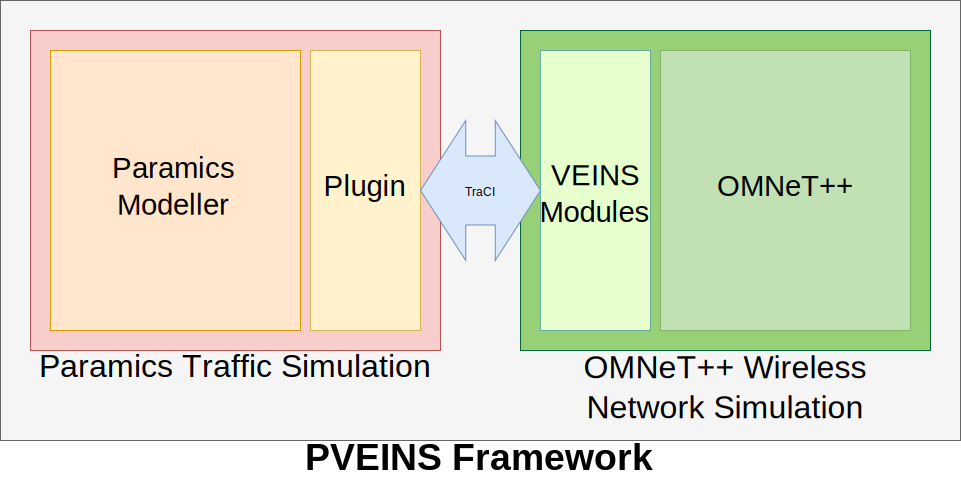
\includegraphics[width=\linewidth]{figuras/PVEINSArch.png}
    \end{column}
    \begin{column}{.3\linewidth}
        \begin{itemize}
            \item Extensible
            \item Mantiene compatibilidad
            \item Facilidad de Uso
            \item Simplifica desarrollo
        \end{itemize}
    \end{column}
\end{columns}
\end{frame}

\begin{frame}{Implementación y Desarrollo}
\begin{columns}
    \begin{column}{.5\linewidth}
        \centering
        \includegraphics[width=.5\linewidth]{figuras/c++.png}
    \end{column}
    \begin{column}{.5\linewidth}
        \centering
        \includegraphics[width=.8\linewidth]{figuras/VisualStudio.png}
    \end{column}
\end{columns}
\end{frame}

\begin{frame}{Implementación y Desarrollo}
\begin{figure}
    \centering
    \includegraphics[width=.5\linewidth]{figuras/modules_pveins.png}
\end{figure}
\end{frame}

\begin{frame}{Implementación y Desarrollo}
\begin{columns}
    \begin{column}{.4\linewidth}
        \begin{itemize}
            \item Desarrollo iterativo.
            \item Buenas prácticas y documentación.
            \item Git.
        \end{itemize}
    \end{column}  
    \begin{column}{.6\linewidth}
        \includegraphics[width=\linewidth]{figuras/poststep_code.png}
    \end{column}    
\end{columns}
\end{frame}

\section{Validación y Resultados}

\begin{frame}{El Escenario}
\begin{columns}
    \begin{column}{.5\linewidth}
        \begin{figure}[p]
            \centering
            \includegraphics[width=\linewidth]{figuras/costanera.png}
        \end{figure}
    \end{column}
    \begin{column}{.5\linewidth}
        \begin{figure}[p]
            \centering
            \includegraphics[width=\linewidth]{figuras/costanera_maps.png}
        \end{figure}
    \end{column}
\end{columns}
\end{frame}

\begin{frame}[standout]
\centering
Demo
\end{frame}

\begin{frame}{Resultados: Nro. Vehículos que alcanzaron destino}
\begin{figure}
    \centering
    \renewcommand{\figurewidth}{\linewidth}
    \renewcommand{\figureheight}{200}
    % This file was created by matplotlib2tikz v0.6.10.
\begin{tikzpicture}

\begin{axis}[
xlabel={Factor de Demanda},
xmin=-0.22, xmax=2.42,
ymin=0, ymax=5000,
width=\figurewidth,
height=\figureheight,
xtick={0.1,1.1,2.1},
xticklabels={20\%,50\%,100\%},
tick align=outside,
tick pos=left,
xmajorgrids,
x grid style={lightgray, opacity=0.7},
ymajorgrids,
y grid style={lightgray, opacity=0.7},
axis line style={black, opacity=0.0},
legend cell align={left},
legend style={at={(0.03,0.97)}, anchor=north west, draw=white!80.0!black, fill=white!89.803921568627459!black},
legend entries={{Sin comunicaci\'on},{Con comunicaci\'on}}
]
\addlegendimage{ybar,ybar legend,fill=red,draw opacity=0};
\draw[fill=red,draw opacity=0] (axis cs:-0.1,0) rectangle (axis cs:0.1,985);
\draw[fill=red,draw opacity=0] (axis cs:0.9,0) rectangle (axis cs:1.1,2441);
\draw[fill=red,draw opacity=0] (axis cs:1.9,0) rectangle (axis cs:2.1,3801);
\addlegendimage{ybar,ybar legend,fill=blue,draw opacity=0};
\draw[fill=blue,draw opacity=0] (axis cs:0.1,0) rectangle (axis cs:0.3,1009);
\draw[fill=blue,draw opacity=0] (axis cs:1.1,0) rectangle (axis cs:1.3,2512);
\draw[fill=blue,draw opacity=0] (axis cs:2.1,0) rectangle (axis cs:2.3,3858);
\node at (axis cs:-0.05,1025)[
scale=1.0,
anchor=west,
text=black,
rotate=45.0
]{ 985};
\node at (axis cs:0.95,2481)[
scale=1.0,
anchor=west,
text=black,
rotate=45.0
]{ 2441};
\node at (axis cs:1.95,3841)[
scale=1.0,
anchor=west,
text=black,
rotate=45.0
]{ 3801};
\node at (axis cs:0.15,1049)[
scale=1.0,
anchor=west,
text=black,
rotate=45.0
]{ 1009};
\node at (axis cs:1.15,2552)[
scale=1.0,
anchor=west,
text=black,
rotate=45.0
]{ 2512};
\node at (axis cs:2.15,3898)[
scale=1.0,
anchor=west,
text=black,
rotate=45.0
]{ 3858};
\end{axis}

\end{tikzpicture}
\end{figure}
\end{frame}

\begin{frame}{Resultados: Distancia vs Tiempo}
\begin{figure}
    \centering
    \renewcommand{\figurewidth}{\linewidth}
    \renewcommand{\figureheight}{165}
    \input{figuras/per00per10_timedistance.tex}
\end{figure}
\end{frame}

\begin{frame}{Resultados: Duración de la Simulación}
\begin{figure}
    \centering
    \renewcommand{\figurewidth}{\linewidth}
    \renewcommand{\figureheight}{165}
    \input{figuras/n_vhcs_vs_time.tex}
\end{figure}
\end{frame}

\section{Conclusiones}
\begin{frame}{Cumplimiento de Objetivos}
\centering
\begin{minipage}{.8\textwidth}
    \begin{enumerate}\pause
        \item Establecer el estado del arte;\hfill\checkmark\pause
        \item Identificar una solución viable;\hfill\checkmark\pause
        \item Diseñar la solución;\hfill\checkmark\pause
        \item Implementar el mecanismo;\hfill\checkmark\pause
        \item Validar su funcionamiento.\hfill\checkmark
    \end{enumerate}%
\end{minipage}
\end{frame}

\begin{frame}{Aprendizajes y comentarios finales}
\begin{itemize}
    \item Trabajar con software propietario es difícil. \pause
    \item Aprendizaje en un área específica, alejada de lo ``común''. \pause
    \item M. Olguín, C. E. Cortés, S. Céspedes, J. Bustos, \textbf{An Integrated Framework for IVC Simulation under Realistic Transport Environments}, \textit{97th Annual Meeting of the Transportation Research Board}, 2018.
\end{itemize}
\end{frame}

\begin{frame}[standout]
Gracias!
\end{frame}

\begin{frame}{Integrantes}
\begin{columns}
    \begin{column}{.5\textwidth}
        Profesora Guía:\\
        \textbf{Sandra Céspedes, DIE}\\
        \vspace{\belowdisplayskip}
        Comisión:\\
        \textbf{Javier Bustos, DCC}\\
        \textbf{Nancy Hitschfeld, DCC}\\
        \vspace{\belowdisplayskip}
        Mención Adicional:\\
        \textbf{Cristián Cortés, DIC}
    \end{column}%  
    \begin{column}{.5\textwidth}
        \centering
        %\includegraphics[width=0.8\textwidth]{figuras/logo_escudo_png.png}\\
        \includegraphics[height=.25\textheight]{figuras/fcfm_horizontal_png.png}\\
        \vspace{0.05\textheight}
        \includegraphics[height=.25\textheight]{figuras/dcc_antiguo_png.png}\\
        \vspace{0.05\textheight}
        \includegraphics[height=.25\textheight]{figuras/niclabs.png}    
        \note{Presentar miembros comisión.}
    \end{column}
\end{columns}    
\end{frame}

\begin{frame}[c,allowframebreaks]{Referencias}
\printbibliography[heading=none]
\end{frame}

\begin{frame}%[standout]
\begin{quote}
    \centering
    \textbf{``‘Intelligent Transport Systems’ or ‘ITS’ means systems in which information and communication technologies are applied in the field of road transport, including infrastructure, vehicles and users, and in traffic management and mobility management, as well as for interfaces with other modes of transport''\footnote{\textcite{eudirective}}}
\end{quote}
\end{frame}

\begin{frame}{Simuladores de Transporte: Comunicaciones vs Transporte}
\begin{figure}[p]
    \centering
    \includegraphics[width=.8\linewidth]{figuras/popular_trafficsims.png}
    \caption{Simuladores de transporte utilizados en el área de transportes\\(Mubasher \emph{et al.} \autocite{traffic_sim_review})}
\end{figure}
\end{frame}


\begin{frame}{Simuladores de Transporte: Comunicaciones vs Transporte}
\begin{figure}[p]
\centering
\includegraphics[height=.7\textheight]{figuras/trafficsims_comp}
\caption{Simuladores de transporte utilizados en el área de comunicaciones\\(Sommer \emph{et al.} \autocite{sommer_dressler2})}
\label{fig:trafficsimscomp}
\end{figure}
\end{frame}

\begin{frame}{Resultados: Carga sobre el Sistema}
\begin{figure}
    \centering
    \renewcommand{\figurewidth}{\linewidth}
    \renewcommand{\figureheight}{180}
    \input{figuras/system_performance.tex}
\end{figure}
\end{frame}

\begin{frame}{Resultados: Distancia vs CO$^2$}
\begin{figure}
    \centering
    \renewcommand{\figurewidth}{\linewidth}
    \renewcommand{\figureheight}{165}
    \input{figuras/per00per10_co2.tex}
\end{figure}
\end{frame}



\begin{frame}{VEINS}
\begin{columns}
\begin{column}{.3\linewidth}
    \centering
    \textbf{Idea: Reemplazar SUMO...}
\end{column}
\begin{column}{.7\linewidth}
    \centering
    \includegraphics[width=\linewidth]{figuras/veins-arch-nosumo.png}
    \captionof{figure}{Arquitectura de VEINS\\Fuente Sommer \emph{et al.} \autocite{sommer_german_dressler}}
\end{column}
\end{columns}
\end{frame}

\begin{frame}{VEINS}
\begin{columns}
\begin{column}{.3\linewidth}
\centering
\textbf{... con Paramics!}
\end{column}
\begin{column}{.7\linewidth}
\centering
\includegraphics[width=\linewidth]{figuras/veins-arch-paramics.png}
\captionof{figure}{Arquitectura de VEINS\\Fuente Sommer \emph{et al.} \autocite{sommer_german_dressler}}
\end{column}
\end{columns}
\end{frame}

\end{document}